Известная Пловдивская шоколадница Бонни хочет разрезать плитку шоколада с изюмом. Плитка имеет прямоугольную форму и состоит из одиночных квадратных кусочков. Кусочки выровнены параллельно краям плитки таким образом, что они формируют $N$ строк и $M$ столбцов, всего получается $N \cdot M$ кусочков. На каждом из кусочков имеется одна или более изюминок, и никакая изюминка не лежит между кусочками и не пересекает разрез между ними.

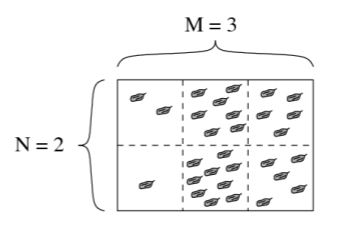
\includegraphics{raisins1.png}

Изначально плитка шоколада представляет собой единое целое. Бонни хочет разрезать её на все меньшие и меньшие части, пока она, наконец, не разрежет всю плитку шоколада на $N\cdot M$ одиночных кусочков. Поскольку Бонни очень занята, она попросила своего ассистента Петра помочь разрезать плитку шоколада. Пётр делает только прямые разрезы от края до края части. Он хочет, чтобы ему платили за каждый разрез, который он сделает. У Бонни совсем нет денег, но у неё осталось бесконечное количество изюминок, и она собирается расплачиваться с Петром изюмом. Петра это устраивает, но при следующем условии: каждый раз, когда он разрезает часть шоколада на две меньших части, он получает столько же изюминок, сколько было на исходной части. 

Бонни хочет заплатить Петру как можно меньше. Она знает, сколько изюминок находится на
каждом из $N\cdot M$ кусочков. Она может выбрать порядок, в котором даёт Петру остающиеся части, и она также может говорить Петру, какие именно разрезы делать (горизонтальные или
вертикальные) и в каком именно месте. Помогите Бонни решить, как разрезать плитку шоколада на одиночные кусочки таким образом, чтобы расплатиться с Петром как можно меньшим
количеством изюминок.

Напишите программу, которая по заданному количеству изюминок на каждом из одиночных
кусочков определяет минимальное количество изюминок, которым Бонни должна расплатиться с
Петром.